\documentclass[12pt]{article}
\usepackage{geometry}
\geometry{left=1in,right=0.75in,top=1in,bottom=1in}
\usepackage{color}
\usepackage{longtable}
% \usepackage{hyperref}
\usepackage[hidelinks]{hyperref}
\usepackage{float}
\usepackage[toc,page,title,titletoc,header]{appendix}
\usepackage[font=small,labelfont=bf]{caption}
\usepackage{ifthen}
\usepackage{amsmath,amssymb,amsthm}
\usepackage{xcolor}

\usepackage{fancyhdr}
\usepackage{minted}
\usepackage{booktabs}
\usepackage{indentfirst}
\usepackage{multirow}
\usepackage{tikz}
\usepackage{pgfplots}
\usepackage{graphicx}
\usepackage{tabularx}
\usepackage{lastpage}
\usepackage{cite}
% \usepackage[backend=bibtex]{biblatex}
\usetikzlibrary{positioning}

\newcommand{\Problem}{A}
\newcommand{\Team}{2122216}

\numberwithin{equation}{section}
\graphicspath{{figures/}}
\lhead{Team \Team}
\rhead{}
\cfoot{}

% \setlength{\parindent}{2em}
\setlength{\parskip}{0.5em}

\theoremstyle{definition}
\newtheorem{definition}{\noindent Assumption}

\pagestyle{fancy}
\rhead{Page \thepage\ of \pageref{LastPage}}

%
\begin{document}

\thispagestyle{empty}
\vspace*{-16ex}
\centerline{
	\begin{tabular}{*3{c}}
		\parbox[t]{0.3\linewidth}{
		\begin{center}\textbf{Problem Chosen} \\
				\Large \textcolor{red}{\Problem}
			\end{center}} &
		\parbox[t]{0.3\linewidth}{
		\begin{center}
				\textbf{2020\\ MCM/ICM\\ Summary Sheet}
			\end{center}} &
		\parbox[t]{0.3\linewidth}{
		\begin{center}
				\textbf{Team Control Number} \\
				\Large \textcolor{red}{\Team}
			\end{center}}   \\
		\hline
	\end{tabular}
}

% Summary
\begin{center}
    \Large\bf Competition, Adaptation and Biodiversity:\\How Fungi Support Our Biosphere
\end{center}

Fungi are prominent components of terrestrial ecosystems in terms of biomass and diversity, and they influence almost every aspect of terrestrial ecosystem functioning. They are the dominant decomposers of organic plant material, with direct consequences for global carbon and nutrient dynamics \cite{Maynard-data}.

In this literature, based on the experimental results of fungi traits provided by Daniel S. Maynard et al., and that of fungi decomposition rate provided by Nicky Lustenhouwer et al., we discussed the decay ability of fungi community, and how environmental conditions affect it. The problem is separated into 4 parts.

Firstly, we construct the model describing the relation between the decomposition rate and hyphal extension rate, moisture tolerance for fungi isolate with straightforward linear regression fitting. The decay ability of a fungi community with respect to the community-weighted extension rate is also specified.

Secondly, we extend the traditional \textbf{Lotka-Volterra model} to multispecific case, and further adapted the equation for the fungi community incorporating hyphal extension rate and moisture tolerance.

Thirdly, we introduced \textbf{Markov chain} model to interspecific competitive biological configuration, and inferred the homeostasis of the fungi community. The attempt of applying a time discrete, state status discrete model to a continuous circumstance is bold and novel.

Finally, we build the model describing how environmental conditions affect the fungi community, and specified the relation between the range of variation of moisture in the local environment and fungi hyphal extension rate.

The models are combined together to form an intact solution for predicting the decay ability of a fungi community. Based on this, we discovered that certain combinations of fungi species can persist in corresponding climatic conditions stably, and may boost the decay ability compared with community merely consists of more combative fungi and with less biodiversity. As the environmental conditions changes, the fungi community may be affected intensively in short term, but in the perspective of long term, the fungi community will reach new homeostasis depends on the environmental conditions. In addition to this, larger biodiversity also means the community is more robust against  the variability in the local environment.

\begin{center}
    \textbf{Keywords:} fungi, interspecific competition, biological degredation, biodiversity
\end{center}


% Table of Contents
\clearpage
% \setcounter{page}{1}
\tableofcontents


% Contents
\section{Introduction}\label{sec:intro}

\subsection{Problem Background}

The carbon cycle describes the process of the exchange of carbon throughout the geochemical cycle of the Earth, and is a vital component for life on the planet. One key component of this part of the process is the decomposition of plant material and woody fibers.

Some of the key agents in decomposing woody fibers are fungi. The authors of a recent research article on wood decomposition by fungi identified fungi traits that determine decomposition rates and also noted links between certain traits. In particular, the slow growing strains of fungi tend to be better able to survive and grow in the presence of environmental changes with respect to moisture and temperature, while the faster growing strains tend to be less robust to the same changes.

\subsection{Problem Restatement}
\begin{itemize}
\item Build a mathematical model that describes the breakdown of ground litter and woody fibers through fungal activity in the presence of multiple species of fungi.
\item In your model, incorporate the interactions between different species of fungi, which have different growth rates and different moisture tolerances.
\item Provide an analysis of the model and describe the interactions between the different types of fungi. The dynamics of the interactions should be characterized and described including both short- and long-term trends. Your analysis should examine the sensitivity to rapid fluctuations in the environment, and you should determine the overall impact of changing atmospheric trends to assess the impact of variation of local weather patterns.
\item Include predictions about the relative advantages and disadvantages for each species and combinations of species likely to persist, and do so for different environments including arid, semi-arid, temperate, arboreal, and tropical rain forests.
\item Describe how the diversity of fungal communities of a system impacts the overall efficiency of a system with respect to the breakdown of ground litter. Predict the importance and role of biodiversity in the presence of different degrees of variability in the local environment.
\end{itemize}
\subsection{Our Work}

\begin{figure}\caption{Work flow of our modelling}
    \begin{center}
        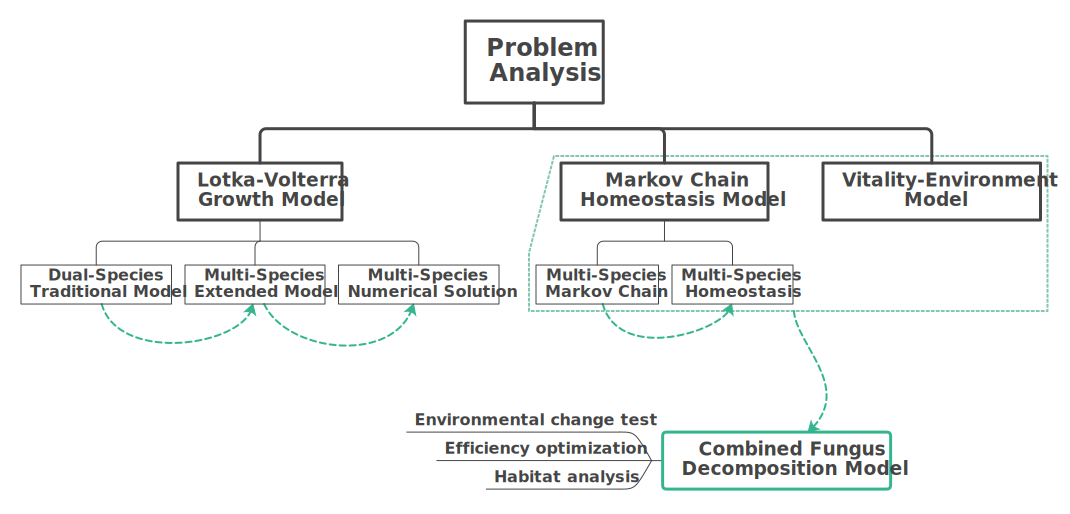
\includegraphics[width=\columnwidth]{workflow.pdf}
    \end{center}\end{figure}

\section{Assumptions and Notations}\label{sec:assump}

Our model is based on several approximate but reasonable assumptions. For a certain ecological configuration in restricted region, such as the decomposition process of a log dominated by fungus, it is equivalent for considering the quantity of fungus individual, biomass or population density. Therefore, our modeling is based on the population density of each species of fungus.

\paragraph{Assumption 1}: Under fixed environmental condition, the ability of a fungi population for decomposing ground litter and woody fibers is proportional to its population density, the coefficient of which is a constant.

\textbf{Justification}: The rate of decomposition is rather complicated, and with temporal memory, since it is in fact determined by the total amount of enzyme exists. In addition, two or more categories of enzyme may interact with each other or together to boost or resist the decomposition reaction. However, to simplify the problem, we ignore such mechanisms, and include all the other factors that affects the biological vitality of the fungus in a single parameter.

\paragraph{Assumption 2}: The constant mentioned above, hence the ability of different fungus species for decomposition, is only related to environmental temperature and humidity.

\textbf{Justification} According to the problem given and other researches, temperature and humidity are the two dominating factors for fungus community, and should be taken into consideration.

\paragraph{Assumption 3} The vital activity of fungus community, that is, the product of metabolization, has no effect on the environment humidity and temperature.

\textbf{Justification} In nature circumstances, the decomposition process happens in open air, the heat and moisture produced or absorbed by fungus can be promptly carried off or replenished  by the external environment, hence the local environment dominates the conditions of the growth of fungus community.

\paragraph{Assumption 4} The decomposition is dominated by the fungus community, and no other species have effect on the system.

\paragraph{Assumption 5} The inter-species relation among the populations in the community is merely competition.

\textbf{Justification} Other inter-species relations such as mutualism, parasitism and predation are rarely seen among fungus. Considering only competition enables us to utilize existed models.

\paragraph{}
Based on these assumptions, we defined the following notations in modeling.

\paragraph{}
\textbf{Assumption 3}: The

\textbf{Justification}: If

\begin{center}\begin{tabular}{ccc}
    \toprule
    Symbol & Definition & Unit \\
    \midrule
    a & b & c \\
    \bottomrule
\end{tabular}\end{center}
\section{Decomposition Rate with Respect to Dominant Fungi Traits}\label{sec:rate}

In this problem, the \textbf{hyphal extension rate} and \textbf{moisture tolerance} are the two basic dominating traits we need to consider in modeling the decay ability of the fungi community.

\subsection{Decomposition  rate model regarding  hyphal  extension  rate,  moisturetolerance and competitive ranking}


\begin{figure}
    \centering
    \begin{minipage}[t]{0.48\textwidth}
        \centering
        \includegraphics[width=0.8\textwidth]{figure1.jpg}
        \caption{The relationship between the hyphal extension rate (mm/day) of various fungi and the resulting wood decomposition rate (\% mass loss over 122 days) at various temperatures.}\label{fig:hyphal}
    \end{minipage}
    \begin{minipage}[t]{0.48\textwidth}
        \centering
        \includegraphics[width=0.8\textwidth]{figure2.jpg}
        \caption{The relationship between the moisture tolerance (difference of each isolate’s competitive ranking and their moisture niche width, both scaled to $[0,1]$) of various fungi and the resulting wood decomposition rate (\% mass loss over 122 days, log transformed).}\label{fig:moisture}
    \end{minipage}
\end{figure}
    

From Figure \ref{fig:hyphal} and Figure \ref{fig:moisture}, it is observed that the relation between the decomposition rate and hyphal extension rate, as well as between the log transformed decomposition rate and relative moisture tolerance are approximately linear.

\begin{equation}
    \left\{\begin{aligned} &
        D = k_1r + b_1 \\ &
        \ln D = k_2(c - m) + b_2
    \end{aligned}\right.
\end{equation}

Apparently, if the hyphal extension rate is $0$, the composition rate would also be $0$, hence the parameter $b_1$ is intrinsically $0$. The model is further specified as

\begin{equation}\label{eq:decay-ability}
    \left\{\begin{aligned} &
        D = k_1r \\ &
        \ln D = k_2(c - m) + b_2.
    \end{aligned}\right.
\end{equation}

% TODO: tolerance, ranking, width?

Note that, in \ref{fig:moisture}, the $x$-axis variable is not exactly the moisture tolerance (moisture niche width), instead is the difference of each isolate’s competitive ranking and their moisture niche width, in range $[-1, 1]$. Hence in the model, competitive ranking $c$ is taken into consideration.


\subsection{Decomposition rate data fitting for single fungus isolate}

Based on the traits data of various species of fungus provided in [], and the resulting experimental 

The fitting result is shown below



% TODO: cite the references, and label where the data comes from

\subsection{Extending the model to multi-species system}

\begin{figure}\label{fig:community}
    \begin{minipage}{0.4\textwidth}
        \includegraphics[width=\textwidth]{figure3.png}
    \end{minipage}
    \begin{minipage}{0.5\textwidth}
        \caption{The decomposition of logs increases with the hyphal extension rate of the fungal community that colonized them. This figure is adapted from []}
    \end{minipage}
\end{figure}

For multi-species case, according to [], the decomposition of logs increases with the hyphal extension rate of the community, and is approximately characterized by a linear model with respect to the community-weighted mean extension rate. Therefore, in order to describe the decay ability of a community consists of multiple species of fungus, the relative quantity relation between of each isolate in the community is necessary.

The decay ability of a fungi community can be described quantitatively as the following expression.

\begin{equation}\label{eq:dcomm}
    D_\text{comm} =
    k_3\bar{r} =
    k_3\frac{r_1x_1 + \cdots + r_nx_n}{x_1 + \cdots + x_n} =
    k_3\dfrac{\sum_{i=1}^n r_ix_i}{\sum_{i=1}^n x_i}.
\end{equation}

% TODO: cite the references, and label where the data comes from

With the data presented in [], the coefficient $k_3$ is roughly determined as [] for 3 years of decay, [] for 5 years. 

% TODO: relation with time

Research conducted in [] presents the data obtained from experimental results on various wood substrate for 3 years or 5 years.

For solving this model for practical prediction of the decay ability of fungi community, each $x_i$ needs to be specified. This part is discussed in the following sections.

\section{Competition Model of the Growth of Fungi Community}\label{sec:LV}


\subsection{Traditional Lotka-Volterra model for dual-species system}

In the early twentieth century, Alfred Lotka and Vito Volterra simultaneously derived a model that described how competition affects population growth from the perspective of differential equations, which is now known as the Lotka-Volterra, or LV model. \cite{LV-model}

First, for single population, if the resources are sufficient enough, the population size, or similarly, density, is expected to grow in the form of

\begin{equation}\label{eq:exp}
    \frac{\mathrm{d}x_1}{\mathrm{d}t} = r_1x_1.
\end{equation}

In which, the intrinsic rate of increase $r$ is the per capita growth rate that could potentially be realized by a fungus population. However, unlimited growth is impossible in reality, environment itself has retardant effect on the population. Take the bounded carrying capacity into consideration, obtains

\begin{equation}\label{eq:logistic}
    \frac{\mathrm{d}x_1}{\mathrm{d}t} =
    r_1x_1\left(1 - \frac{x_1}{K_1}\right).
\end{equation}

The extra term places a limit on exponential growth, and the resulting equation represents the logistic growth.

In a dual-species system, the resistance against the growth of one population comes not only from the environment, but also another specie. It is natural that, when specie 2 has larger population density, specie 1 will be in face of larger competitive pressure, and similar for species 2. Such notion is also capable for intra-specie competition. Combining the inter-species and intr-specie competition into \eqref{eq:logistic}, obtains the differential equations set

\begin{equation}\label{eq:lv-dual}
    \left\{\begin{aligned}     &
        \frac{\mathrm{d}x_1}{\mathrm{d}t} =
        r_1x_1\left(1 - \frac{\alpha_{11}x_1 + \alpha_{12}x_2}{K_1}\right) \\ &
        \frac{\mathrm{d}x_2}{\mathrm{d}t} =
        r_2x_2\left(1 - \frac{\alpha_{22}x_2 + \alpha_{21}x_1}{K_2}\right).
    \end{aligned}\right.
\end{equation}

Which is the model for dual-species competition. Note that, neither Lotka nor Volterra explained this equation from the perspective of ecology, it is Tilman who made a convincing interpretation. His resource-based model included resources requirement, consumption and supply, which is concise and rigorous but not the topic of this literature. \cite{Tilman}


\subsection{Extended Lotka-Volterra model for multi-species}

Based on LV model, we extended \eqref{eq:lv-dual} to a multi-species system with $n$ various populations.

\begin{equation}\label{eq:lv-multi}
    \left\{\begin{aligned}     &
    \frac{\mathrm{d}x_1}{\mathrm{d}t} =
    r_1x_1\left(1 - \frac{\sum_{j=1}^n \alpha_{1j}x_j}{K_1}\right) \\ & \cdots \\ &
    \frac{\mathrm{d}x_i}{\mathrm{d}t} =
    r_ix_i\left(1 - \frac{\sum_{j=1}^n \alpha_{ij}x_j}{K_i}\right) \\ & \cdots \\ &
    \frac{\mathrm{d}x_n}{\mathrm{d}t} =
    r_nx_n\left(1 - \frac{\sum_{j=1}^n \alpha_{nj}x_j}{K_n}\right)
    \end{aligned}\right.
\end{equation}

The equations set can be simplified with matrix differential equations as

\begin{equation}\label{eq:lv-mat}
    \frac{\mathrm{d}\boldsymbol{x}}{\mathrm{d}t} =
    \boldsymbol{r}\cdot\boldsymbol{x}
    \left[\boldsymbol{1} - (\boldsymbol{Ax})\cdot\hat{\boldsymbol{K}}\right].
\end{equation}

In which the matrix $\hat{\boldsymbol{K}}$ is the element-wise reciprocal of $\boldsymbol{K}$, that is, $\hat{\boldsymbol{K}}_{ij}\boldsymbol{K}_{ij} = 1$. 

The growth process of fungus community considering competition is characterized by this first-order linear ordinary differential equations group, with $n$ unknown functions. Note that while the analytical can be difficult to be found, we can still figure out the development of the system using computer numerically.

% Consider a quad-species system, with the parameters shown in table \ref{tb:quad-para}.

% \begin{table}
%     \begin{center}
%         \caption{The parameters}
%         \begin{tabular}{c|cccccc}
%             \toprule
%                   & $r_i$ & $K_i$ & $\alpha_{i1}$ & $\alpha_{i2}$ & $\alpha_{i3}$ & $\alpha_{i4}$ \\
%             \midrule
%             $x_1$ &       &       &               &               &               &               \\
%             $x_2$ &       &       &               &               &               &               \\
%             $x_3$ &       &       &               &               &               &               \\
%             $x_4$ &       &       &               &               &               &               \\
%             \bottomrule
%         \end{tabular}\label{tb:quad-para}
%     \end{center}
% \end{table}

% TODO: If possible, give a solution example


\subsection{Adaptive Lotka-Volterra model for fungi community}

As shown in \eqref{eq:lv-mat}, a significant drawback of LV model is that, in total $n^2 + n$ extra defined parameters, symbolizing the stress exerted from each specie onto each another and the carrying capacity of the environment for each specie are needed. It would be impractical for our model if such amount of factors without support from experimental result need to be considered.

\begin{definition}
    The stress from other species of fungi can be characterized by the ratio of the product of relative moisture tolerance and biomass of the two species, and normalized with an exponential function.
    \textbf{Justification} The relative moisture tolerance is defined as the difference of each isolate’s competitive ranking and their moisture niche width, indicating the significant tolerance-dominance trade-off property in the competition of fungi. While incorporating the effect of multiple species, the form of the differential equations are roughly consistent with LV model.
\end{definition}

Considering features of various types of fungi with available data, and the compatibility to the composition rate model constructed, traditional LV model in dual-species case is redefined to adapt the fungi community circumstances as follows.

\begin{equation}
    \left\{\begin{aligned}         &
        \frac{\mathrm{d}x_1}{\mathrm{d}t} =
        r_1x_1\exp\left(
        1 - \frac{m_1x_1}{m_1x_1}\cdot
        \frac{m_2x_2}{m_1x_1}
        \right) \\ &
        \frac{\mathrm{d}x_2}{\mathrm{d}t} =
        r_2x_2\exp\left(
        1 - \frac{m_1x_1}{m_2x_2}\cdot
        \frac{m_2x_2}{m_2x_2}
        \right)
    \end{aligned}\right.
\end{equation}

When extended to multiple species, we have

\begin{equation}
    \left\{\begin{aligned}         &
        \frac{\mathrm{d}x_1}{\mathrm{d}t} =
        r_1x_1\exp\left(
            1 - \frac{m_1x_1}{m_1x_1}\cdots
            \frac{m_nx_n}{m_1x_1}
        \right) \\ & \cdots \\ &
        \frac{\mathrm{d}x_i}{\mathrm{d}t} =
        r_ix_i\exp\left(
            1 - \frac{m_1x_1}{m_ix_i}\cdots
            \frac{m_jx_j}{m_ix_i}\cdots
            \frac{m_nx_n}{m_ix_i}
        \right) \\ & \cdots \\ &
        \frac{\mathrm{d}x_n}{\mathrm{d}t} =
        r_nx_n\exp\left(
            1 - \frac{m_1x_1}{m_nx_n}\cdots
            \frac{m_nx_n}{m_nx_n}
        \right).
    \end{aligned}\right.
\end{equation}

Or simply expressed as

\begin{equation}\label{eq:LV-adapt}
    \frac{\mathrm{d}x_i}{\mathrm{d}t} =
    r_ix_i\exp\left(
            1 - \frac{\prod_{j=1}^n m_j}{m_i^n}\cdot
            \frac{\prod_{j=1}^n x_j}{x_i^n}
        \right).
\end{equation}

% TODO: simulate numerical solution of a multi-species case 

\section{Homeostasis of the Community with Markov Chain Model}\label{sec:markov}

% TODO: Cite references

\subsection{Feasibility of utilizing Markov chain model in fungus community}

Since it is presumably impractical for finding the symbolic solution of the LV model, Markov chain model is introduced for predicting the stable state, that is, the relatively static composition of the fungus populations density in the community.

\begin{definition}
    Once the community component is stabilized, if possible, the population density of each fungi specie interchange in a rate proportional to its own population density, the coefficient is a constant.
    \textbf{Justification} Though the Markov chain model is based on discrete time and state space, since the stable state is all we concerned in this attempt, we can still utilize such notion.
\end{definition}


\begin{figure}\caption{A Markov chain diagram containing 3 fungi species}\label{fig:markov3}
    \begin{center}
        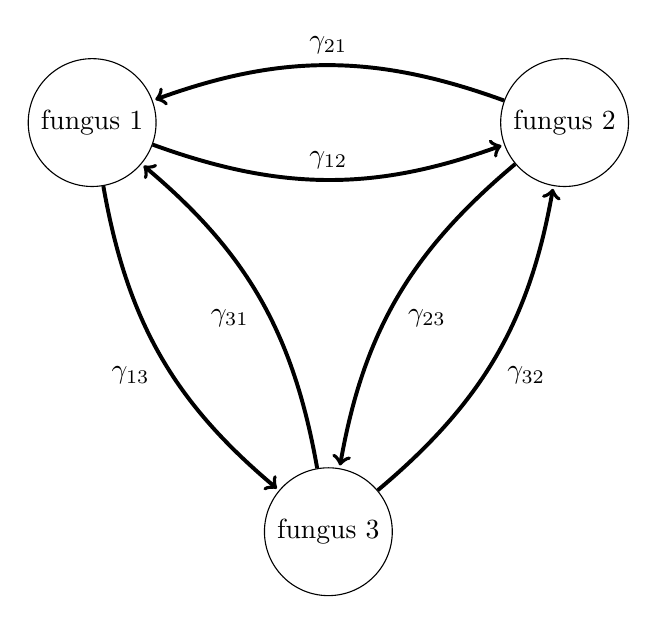
\begin{tikzpicture}
            \node[draw, circle] at (0, 0)     (1)     {fungus 1};
            \node[draw, circle] at (6, 0)     (2)     {fungus 2};
            \node[draw, circle] at (3, -5.196) (3) {fungus 3};
    
            \draw[every loop, auto=right, line width=0.5mm]
                (1) edge[bend right=20]            node {$\gamma_{13}$} (3)
                (1) edge[bend right=20, auto=left] node {$\gamma_{12}$} (2)
                (2) edge[bend right=20]            node {$\gamma_{21}$} (1)
                (2) edge[bend right=20, auto=left] node {$\gamma_{23}$} (3)
                (3) edge[bend right=20]            node {$\gamma_{32}$} (2)
                (3) edge[bend right=20, auto=left] node {$\gamma_{31}$} (1);
        \end{tikzpicture}
    \end{center}
\end{figure}


\subsection{Constructing Markov chain for fungus community}

Consider a given time interval $T$, and the population density of each fungus species at time $t$ is denoted as $\boldsymbol{x}(t) = [x_1(t), x_2(t), \cdots, x_n(t)]^T$. In the evolution process of the community, at each time interval, a specific percentage of fungi $i$ is remained, and others can be considered as transformed into population density of other species of fungus.

For a simple dual-species system, such transition relation can be expressed as

\begin{equation}
    \left\{\begin{aligned} &
        x_1(t+T) = \gamma_{11}x_1(t) + \gamma_{21}x_2(t) \\ &
        x_2(t+T) = \gamma_{22}x_2(t) + \gamma_{12}x_1(t)
    \end{aligned}\right..
\end{equation}

More generally, in an $n$-species community, the system is characterized by

\begin{equation}
    \left\{\begin{aligned} &
        x_1(t+T) = \gamma_{11}x_1(t) + \cdots + \gamma_{n1}x_n(t) \\ & \cdots \\ &
        x_i(t+T) = \sum_{j=1}^n \gamma_{ij}x_j \\ & \cdots \\ &
        x_n(t+T) = \gamma_{n1}x_1(t) + \cdots + \gamma_{nn}x_n(t).
    \end{aligned}\right.
\end{equation}

Which can be further simplified with matrix notation.

\begin{equation}\label{eq:trans}
    \boldsymbol{x}(t+T) = \boldsymbol{x}(t)\boldsymbol{Y}.
\end{equation}

In which, the matrix $\boldsymbol{Y}_{n\times n}$ is defined to be the transition matrix of the system, with element $\gamma_{ij}$ denoting the transition rate from fungus specie $i$ to $j$.

\begin{equation}
    \boldsymbol{Y} =
    \begin{bmatrix}
        \gamma_{11} & \gamma_{12} & \cdots & \gamma_{1n} \\
        \gamma_{21} & \ddots & & \vdots \\
        \vdots & & \ddots & \vdots \\
        \gamma_{n1} & \cdots & \cdots & \gamma_{nn}
    \end{bmatrix}
\end{equation}

Note that the transition rate in the biological configuration considerably differs from that in stochastic process. In a typical Markov chain model, each element in the transition matrix represents a certain probability of transition or decision towards another state. To implement this model in a continuous mathematical configuration, adjustments must be and evidently can be made to the definition of the population density $x_i$ itself, ensuring that a unit of population density of different species of fungus takes up the same amount of resources in the system. With such adjustment, it is guaranteed that, for each element and row of the transition matrix, we have

\begin{equation}\label{eq:markov-norm}
    \left\{\begin{aligned} &
        \boldsymbol{Y}_{ij} \in [0,\ 1],\ i,\ j\in\{1,\ 2,\ \cdots,\ n\} \\ &
        \sum_{j=1}^n \boldsymbol{Y}_{ij} = 1,\ i\in\{1,\ 2,\ \cdots,\ n\}.
    \end{aligned}\right.
\end{equation}

In addition, though during the growth process of the populations, and in macroscopic view the early stage of the decomposition, the transition matrix may not satisfy condition \eqref{eq:markov-norm}, and the sum of the rows could possibly even vary with time, it is shown that the final homeostasis is only related to the transition matrix after the community enters Markov process.


\subsection{Incorporate hyphal extension rate and moisture tolerance}

To model the system of fungi community, the transition matrix is further specified as follows in order to incorporate traits we concerned.

\begin{equation}\label{eq:gamma}
    \gamma_{ij} =
    \mathrm{Softmax}\left(1 - \frac{r_i}{r_j}\right) =
    \frac{e^{1 - r_i / r_j}}{\sum_{k=1}^n e^{1 - r_i / r_k}} =
    \frac{e^{- r_i / r_j}}{\sum_{k=1}^n e^{- r_i / r_k}}.
\end{equation}

% In another word, each row in the transition matrix is identical, and the element at each row can be expressed as

% \begin{equation}
%     \pi(j) = \frac{r_j}{\sum_{k=1}^n r_k}.
% \end{equation}

In which the $\mathrm{Softmax}$ is for normalizing the data. The hyphal extension rate is a significant trait characterizing the \textbf{combative ability} of fungus, the ratio represents at what rate a fungus will be replaced another fungus isolate. It can be easily verified that, definition \eqref{eq:gamma} is normalized for keeping consistent with prerequisite \eqref{eq:markov-norm}.

The final homeostasis can be expressed simply as

\begin{equation}\label{eq:markov-limit}
    \boldsymbol{\pi} =
    \boldsymbol{x}(0)\lim_{n\rightarrow\infty}\boldsymbol{Y}^n.
\end{equation}


\subsection{The homeostasis of the system}

% Once the total population density reached the overall carrying capacity of the system, condition \eqref{eq:norm} is automatically satisfied. It is obvious that, according to \eqref{eq:trans}, after $nT$ time, the the population density in the community turns into

% \begin{equation}
%     \boldsymbol{x}(t+nT) =
%     \boldsymbol{Y}\boldsymbol{x}[t+(n-1)T] = \cdots =
%     \boldsymbol{Y}^n\boldsymbol{x}(t).
% \end{equation}

% For solving this model, consider the eigenvalues and eigenvectors of the transition matrix\dots

% \begin{equation}
%     \boldsymbol{Y}\boldsymbol{z} = \lambda\boldsymbol{z} \Rightarrow
% \end{equation}

In a Markov process, the final homeostasis is only related to the transition matrix as shown in \eqref{eq:markov-limit}, but cannot be explicitly expressed.We postulate a quad-species fungi community, among them two in the top and two in the bottom of the competitive ranking, to visualize and verify this model.

The traits value of the four fungi is shown in table \ref{tb:markov-4}, and the transition matrix is

\[\begin{bmatrix}
    0.45253 & 0.54712 & 0.00000 & 0.00035 \\
    0.44167 & 0.55827 & 0.00000 & 0.00006 \\
    0.32586 & 0.32935 & 0.12678 & 0.21801 \\
    0.38964 & 0.39879 & 0.04959 & 0.16198
\end{bmatrix}\]

\begin{table}\caption{The four species chosen in verifying the model}\label{tb:markov-4}
    \centering
    \begin{tabular}{c|cc}
        \toprule
        Specie & Competitive Ranking & Hyphal Extension Rate \\
        \midrule
        Phlebia acerina MR4280 B9G & 1 & 8.75 \\
        Phlebiopsis flavidoalba FP150451 A8G & 0.9864 & 10.8 \\
        Armillaria gallica HHB12551 C6C & 0 & 0.49 \\
        Armillaria tabescens TJV93 261 A1E & 0 & 1.07 \\
        \bottomrule
    \end{tabular}
\end{table}

As the iteration proceeds, the system reached the homeostasis gradually, and dominant species substitute weaker species completely in the end.

\begin{figure}\label{fig:markov-4}
    \begin{minipage}{0.6\textwidth}
        \includegraphics[width=\textwidth]{markov-4.png}
    \end{minipage}
    \begin{minipage}{0.4\textwidth}
        \caption{The community composition of a quad-species system, after several iteration, the relative biomass reaches homeostasis. 1 - Phlebia acerina, 2 - Phlebiopsis flavidoalba, 3 - Armillaria gallica, 4 - Armillaria tabescens}
    \end{minipage}
\end{figure}

\section{Environmental Effect on the Decay Ability of the Community}\label{sec:env}

The purpose of this section, is to describe the environment affect the decomposition ability of a fungi community.

Since in this literature, moisture tolerance is the only trait of fungi concerned related to environment, we focus on how environment interact with this property.

\subsection{Environmental impact on the hyphal extension rate}

Moisture tolerance is defined as the difference of each isolate’s competitive ranking and their moisture niche width. Competitive ranking can be obtained through pair wise competition experiment, and won't be affect by environment conditions since it is a relative ranking relation between species. Moisture niche width is the immediate property representing how tolerant a specie can be against varying environmental moisture condition, which is defined as the difference between the maximum and minimum moisture levels in which half of a fungal community can maintain its fastest growth rate.

According to \eqref{eq:decay-ability}, the hyphal extension rate and moisture niche width are implicitly related, and can be quantified as

\begin{equation}
    k_2(c - d) + b_2 = \ln k_1r \Rightarrow
    r = \frac{1}{k_1} \exp[k_2(c -d) +b_2].
\end{equation}

\begin{definition}
    The hyphal extension rate of fungi community is affected by the moisture range of the environment. When the humidity in the environment fluctuates in a remarkable range, the growth of fungi is depressed. 
    \textbf{Justification} In this model, the community can be treated as a whole, since moisture tolerance only has to do with the niche width, not the optimal moisture condition. The optimal moisture condition and the moisture niche can be varied a lot in a fungi community for different species, but the global trend with respect to the change of environment can be predicted in such assumption.
\end{definition}

Define the moisture range in a certain environment as $w$, then the hyphal extension rate expression can be expressed as

\begin{equation}
    \hat{r} =
    \frac{1}{k_1} \exp[k_2(c -d) +b_2]\cdot
    \frac{d}{w + d}.
\end{equation}

The meaning of the extra factor in the equation is, if the environmental moisture width is exactly zero, then the hyphal extension rate of the community is considered as being right in the optimal moisture width of the system as a whole. Otherwise, if the environmental moisture moisture width is equal to the feature moisture niche width of the community, then the hyphal extension rate is halved, which is consistent with the definition of niche width.

In addition, if the initial hyphal extension rate in a certain condition is available and denoted as $r_0$, we can predict the same trait in other environment as

\begin{equation}\label{eq:env}
    \hat{r} = \frac{d}{w + d}r_0.
\end{equation}

\subsection{Applying the data in various climates}

After collecting and processing climate property data, we can obtain the moisture width of different climate, then apply these data to the model.

\begin{table}[h]\caption{The moisture width $w$ in different environments}
    \centering
    \begin{tabular}{c|ccccc}
        \toprule
        climate        & arid & semi-arid & temperate & arboreal & tropical rain forests \\
        \midrule
        moisture width &      &           &           &          &                       \\
        \bottomrule
    \end{tabular}
\end{table}

\section{Combined Model of the Decay Ability Regarding Environment}\label{sec:com}

In this section, the decay ability model, the growth model describing the composition of the fungi community, and the environmental factors are combined to determine the behaviors of the fungi community in breakdown process.

\subsection{Combining the models}

In \eqref{eq:dcomm}, replace the hyphal extension rate with \eqref{eq:env}, obtains

\begin{equation}\label{eq:dcomm-env}
\hat{D}_\text{comm} =
    k_3\frac{\sum_{i=1}^n \hat{r}_i}x_i{\sum_{i=1}^n x_i} =
    k_3\dfrac{\sum\limits_{i=1}^n \dfrac{d_ir_ix_i}
    {w + d_i}}{\sum\limits_{i=1}^n x_i}.
\end{equation}

In \eqref{eq:LV-adapt}, conduct the same substitution, obtains

\begin{equation}\label{eq:LV-env}
    \frac{\mathrm{d}x_i}{\mathrm{d}t} =
    \frac{d_ir_i}{w + d_i}x_i\exp\left(
            1 - \frac{\prod_{j=1}^n m_j}{m_i^n}\cdot
            \frac{\prod_{j=1}^n x_j}{x_i^n}
        \right).
\end{equation}

Also, the transition matrix redefined in \eqref{eq:gamma} is again transformed into

\begin{equation}\label{eq:markov-env}
    \gamma_{ij} = 
    \frac{\hat{r}_i}{\sum_{k=1}^n \hat{r}_k} =
    \frac{\dfrac{d_ir_{ik}}{w + d_i}}
    {\sum\limits_{k=1}^n \dfrac{d_ir_{ik}}{w + d_i}}.
\end{equation}


Equation \eqref{eq:dcomm-env} determines the ability of a fungi community to decompose ground litter and woody fibers. In which, $r_i$, $d_i$ are the traits of the fungus, $w$ is determined by the environmental condition, $k_3$ is a coefficient and is determined in data fitting as shown in \ref{tb:para-year}. $x_i$ is the only unknown variable representing the biomass of different species of fungus, and can be inferred numerically through \eqref{eq:LV-env}, in which $m_i$ is the trait owned by fungus.



\subsection{Solution of the model at different climatic conditions}

Since a explicit analytical solution cannot be attained from \eqref{eq:LV-env}, yet from model defined in section \ref{sec:markov}, we choose all 34 fungi species with available traits data from [], and evaluate their behaviors under different climatic conditions. For the purpose of brevity, [] model is chosen.

% TODO: which model? do a simulation in secs before to find out
% TODO: write script and solve them! plot!

\section{Analysis}\label{sec:analysis}

\subsection{Sensitivity Analysis}

\subsubsection{xxx}
\subsubsection{xxx}

\subsection{Strengths and Weaknesses}

\section{Conclusions}\label{sec:conclu}

In conclusion, hyphal extension rate and moisture tolerance are positively related to the decay ability of a fungi isolate as well as the community. In a fungi community, the decay ability is determined by its community-weighted hyphal extension rate. The composition of a fungi community in homeostasis can be inferred from Markov chain model or solving adaptive LV-model.

Environmental conditions have affect on the composition of the community, hence alters the decay ability. The larger the varying range of local environmental condition is, the slower the decomposition becomes. Certain species combinations may suitably persis in corresponding climate. In general, biodiversity is positively related to the decay ability. In short term, the fluctuation of environmental conditions may affect the fungi community intensively, however, in long term, the community will reach a new homeostasis.



\newpage
\section*{Competition, Adaptation and Biodiversity:\\How Fungi Support Our Biosphere}

\setcounter{figure}{0}

Fungi are everywhere in the world, not just on a rotten orange, or in yeast essential bread and cake. Fungi together with a series of other microbes plays an important role in the biosphere, know as the \textbf{decomposers}. The normal functionality of biosphere requires both sustained energy and material flow, and the latter one consists of not only essential organic chemical compound such as amino acids and glucose, but also inorganic carbon dioxide. Such material flow is also called the \textbf{carbon cycle}.

\begin{figure}[ht]
    \centering
    \includegraphics[width=0.4\textwidth]{isolate.jpg}
    \caption{Fungi in pair wise competition test. This figure is adopted from ``Consistent trade-offs in fungal trait expression across broad spatial scales" by Daniel S. Maynard et al.}
    \label{fig:decom-hyphal-122d}
\end{figure}

In carbon cycle, the \textbf{producers}, mainly the green plants, are responsible for the fixation of carbon, namely transforming the carbon in carbon dioxide into fixed carbon in organic matter through chemosynthesis, of which the most commonly known one is photosynthesis. Then, the \textbf{consumers} utilize these material for vital activities, some carbon transformed into again into the carbon dioxide, some maintain in consumers.

What would these carbon go? Can they go back to the atmosphere? This is where decomposers play a role. Decomposers decompose the cadavers and excrements, function as the bridge in the carbon cycle. Note that, one of the most important features of carbon cycle is that it was global, the beef, egg and milk consumptions in the US might be related to the depletion of Brazilian rain forests, which is why carbon cycle is significant to us all and more and more researchers are interested in this topic.

As an important category in decomposers, fungi are outstanding participants in the decay process, especially when dealing with ground litter and woody fibers. A recent research presented the mechanism of decay efficiency for fungi community. The decay ability is positively related to the hyphal extension rate and moisture tolerance of a fungus isolate. However, as for a fungi community, the thing is getting more complicated.

\begin{figure}
    \begin{minipage}{0.5\textwidth}
        \centering
        \includegraphics[width=\textwidth]{decom-hyphal-122d.png}
    \end{minipage}
    \begin{minipage}{0.5\textwidth}
        \caption{The relationship between the hyphal extension rate of various fungi and the resulting wood decomposition rate. The hyphal extension rate is the geometrical average of the value tested under 10, 16 and 22 Celsius.}
    \end{minipage}
\end{figure}

The composition of the fungi community can be predicted by the famous Lotka-Volterra model as shown in \eqref{eq:lv}, which indicates that in a multi-species system, each species would exert stress on other species. Tilman interprets that, the intrinsic mechanism is the limitation of certain resources. Generally, the fungus which grows slower, can better tolerate a wide range of environmental conditions. Therefore, some most competitive fungi may attain huge superiority at the start, and replace the less combative fungi completely. Sometime, more tolerant fungi might be able to endure the oppression and gain dominance in the later stages. Such feature determines that, some combinations of fungi may be able to persist and reach a dynamic homeostasis. It is apparent that, these combinations may vary with environmental conditions, you may do your own experiments in the laboratory to find out the ``recipe".

\[
    \label{eq:lv}\tag{$\ast$}
    \frac{\mathrm{d}x_i}{\mathrm{d}t} =
    r_ix_i\left(1 - \frac{\sum_{j=1}^n \alpha_{ij}x_j}{K_i}\right)
\]

Another interesting fact is that, when less competitive species of fungi are introduced to the community, the decay ability of the fungi community may be boosted instead of decreased. This phenomenon can be explained as, different species are preponderant in decomposing at different stages. A large varieties of species, namely the \textbf{biodiversity}, enables the possibility of various combinations. Such combination is relevant to the climatic conditions, resulting unique biodiversity in different geographical areas. Biodiversity also makes the community more variability in face of the variability in local environment.

The global carbon cycle integrates whole biosphere all together, with inconspicuous fungi as a crucial part in it. It is our shared responsibility to restrict carbon emission and protect biodiversity. Biodiversity provides efficiency and robustness to our biosphere. Hope next time you could feel less disgusted when seeing a rotten apple, it might be fungi answering their call!



% References
\newpage
\nocite{*}
\bibliographystyle{plain}
\bibliography{biblo}

% Appendix 
\newpage
\appendixpage
\appendix

\section{Source Code}

The source code for Markov chain model.

\inputminted[linenos=true, frame=single]{python}{codes/appendix.py}


\section{Fungi Traits Data}

The decomposition rate data from \cite{Lustenshouwer}, can be retrieved at \href{https://www.pnas.org/content/pnas/suppl/2020/05/13/1909166117.DCSupplemental/pnas.1909166117.sapp.pdf}{Supplementary Information for A trait-based understanding of wood decomposition by fungi}.

The other fungi traits data from \cite{Maynard-data}, can be retrieved at \href{https://github.com/dsmaynard/fungal_biogeography}{dsmaynard/fungal\_biogeography}.


\end{document}
